\documentclass[10pt]{article}
\usepackage[a4paper,margin=2.0cm]{geometry}
\usepackage{amsmath,amssymb,mathtools}
\usepackage{booktabs}
\usepackage{microtype}
\usepackage{graphicx}
\usepackage{enumitem}
\usepackage{hyperref}
\usepackage{xcolor}
\usepackage{tikz}
\usepackage[backend=biber,style=numeric,sorting=nyt]{biblatex}
\addbibresource{hls_foundations_v01.bib}
\usetikzlibrary{arrows.meta,positioning,fit}
\hypersetup{colorlinks=true,linkcolor=blue!45!black,citecolor=blue!45!black,urlcolor=blue!45!black}
\setlist{nosep,leftmargin=*}
\newcommand{\Ccap}{\mathcal{C}}
\newcommand{\PiC}{\Pi}
\newcommand{\argmax}{\operatorname*{arg\,max}}

\title{\textbf{Heterogeneous Learning Systems: A Minimal Theory of Collective Capability, Organization, and Competence Evolution}}
\author{Francisco Javier Gonz\'alez Serrano\\Universidad Carlos III de Madrid}
\date{Working paper v0.1 --- October 2026}

\begin{document}
\maketitle

\begin{abstract}
Many collective systems contain agents or models with heterogeneous, limited, and distributed competences. Two questions then arise: \emph{who should do what?} and \emph{who should learn what, how, and from whom?} Existing theories provide strong answers to important parts of these questions, including assignment and resource allocation, organizational flexibility, learning by doing, competence development, knowledge transfer, and dynamic optimization. Heterogeneous Learning Systems (HLS) does not seek to replace these theories. It provides a minimal architecture in which they can be composed without conflating heterogeneity, attainable capability, efficient capability, realized organizational value, competence change, future value, and decision relevance. We formalize a static beam that maps distributed competence and organizational conditions into collective capability, and a dynamic beam in which realized action can endogenously change future competence. The same static capability operator is then reused on the future state. This yields a closed organization--development loop with only two essential operators: a collective-capability operator and a competence-transition operator. Minimal analytical and computational ground truths show why each logical distinction is necessary. The resulting framework identifies when richer organization or competence evolution is consequential and when it collapses to a simpler problem. HLS is therefore a theory of the organization and development of heterogeneous collective capability, built by importing established components where they suffice and introducing new structure only where the complete HLS question requires it.
\end{abstract}

\section{Introduction}

Collective problem solving rarely starts from interchangeable agents. Human teams, organizations, autonomous systems, and portfolios of learned models differ in what they can do, how well they can do it, what resources they consume, and how their competences evolve. The central HLS problem is to understand how such a collective should \emph{use} its current competences and how it should \emph{develop} future competences when problems, needs, and constraints may change.

HLS is organized around two questions:
\begin{equation}
\text{Beam 1: Who should do what?}
\end{equation}
\begin{equation}
\text{Beam 2: Who should learn what, how, and from whom?}
\end{equation}
These questions have deep antecedents. The organization of distributed knowledge has long been studied in economics and organization theory \cite{garicano2000}; assignment, specialization, comparative advantage, and resource allocation provide established static machinery; learning by doing and task-specific human capital explain endogenous competence evolution \cite{arrow1962,gibbonswaldman2004,argotemiron2011}; competence-oriented portfolio models explicitly connect present choices to future competence \cite{gutjahr2011,gutjahretal2010multiobjective}; and assignment, learning, transfer, and training have already been studied jointly in specific operational settings \cite{nembhardbentefouet2015,borgonjon2024dynamic}. These are foundations to import, not wheels to reinvent.

The HLS question lies at the level of the complete structure. A heterogeneous competence distribution need not create additional collective capability. Additional attainable outcomes need not improve the efficient frontier. An improved frontier need not have value under the current problem and resource constraints. Likewise, competence change need not change future collective capability; a capability change need not be useful for future problems; and useful future competence need not alter the present decision. HLS keeps these objects separate and asks when the dependencies between them are consequential.

The contribution of this paper is deliberately parsimonious. First, we give a common static language for collective capability under competence structure, problem structure, resource constraints, and admissible organization. Second, we introduce endogenous competence evolution only through realized action. Third, we close the loop by applying the \emph{same} static capability operator to the future competence state and asking whether future organizational value changes the present choice. Fourth, we provide minimal constructive ground truths that expose the null and positive cases of the theory. No new assignment algorithm, learning rule, or dynamic-programming method is claimed.

\section{Relation to Established Theory}

HLS follows a simple methodological rule: \emph{reduce before inventing}. If a required component already exists, it is imported, adapted to the HLS ontology, and assigned a precise role.

\paragraph{Organization of distributed competence.}
Garicano's theory of knowledge organization makes explicit that distributed knowledge and organizational access to that knowledge jointly determine problem-solving capability \cite{garicano2000}. Assignment, specialization, comparative advantage, skill-based allocation, and process flexibility provide mature machinery for deciding how heterogeneous resources are used. HLS imports this family of ideas into a common capability representation rather than proposing a new static assignment theory.

\paragraph{Competence evolution.}
Learning by doing \cite{arrow1962}, task-specific human capital \cite{gibbonswaldman2004}, organizational learning from experience \cite{argotemiron2011}, and transfer of human capital \cite{jovanovicnyarko1995} provide established mechanisms by which activity and experience can alter future competence. HLS abstracts these mechanisms into a competence transition; it does not require any particular learning mechanism at the foundational level.

\paragraph{Joint operation and development.}
The interaction itself is also not unprecedented. Dynamic project selection can account for competence development \cite{gutjahr2011}; project selection can be evaluated with competence-oriented multiobjective criteria \cite{gutjahretal2010multiobjective}; assignment policies can include learning by doing and knowledge transfer \cite{nembhardbentefouet2015}; and staffing decisions can explicitly account for dynamic learning and training \cite{borgonjon2024dynamic}. These works demonstrate that operation and development can interact in concrete domains. HLS seeks the domain-independent structure needed to state when such interaction changes collective capability, value, or decisions.

\paragraph{Dynamic optimization.}
Once states, actions, rewards, and transitions are specified, continuation value and dynamic programming are standard. HLS uses this machinery. Its purpose is not to replace dynamic programming, but to specify the competence--organization structure on which dynamic optimization acts and to distinguish physical competence change from collective and decision-relevant consequences.

\section{HLS Setting}

Let $S$ denote the competence structure of a collective, $P$ the problem or demand structure, $B$ the operational constraints or resource budget, and $\Pi$ an admissible class of organizational policies. A policy $\pi\in\Pi$ is a decision rule; $a$ is the action or organizational use actually realized under that rule; and $z$ is the resulting collective outcome. We retain the distinction
\begin{equation}
\pi \neq a,
\end{equation}
because future competence may depend on what is actually done rather than on the nominal policy that selected it.

The static chain is
\begin{equation}
(S,P,B,\Pi) \longrightarrow \pi \longrightarrow a \longrightarrow z.
\end{equation}

\subsection{T0: feasible capability}

For fixed $(S,P,B,\Pi)$, define the attainable collective outcome set
\begin{equation}
\mathcal{F}_{\Pi}(S,P,B)
 = \{z:\exists\,\pi\in\Pi\text{ whose realized action attains }z\},
\end{equation}
and let
\begin{equation}
\Ccap_{\Pi}(S,P,B)
 = \operatorname{Eff}\bigl(\mathcal{F}_{\Pi}(S,P,B)\bigr)
\end{equation}
denote the relevant efficient collective capability. When a scalar operating criterion is required, let
\begin{equation}
V(S;P,B,\Pi)
\end{equation}
be the value obtained from that capability under the specified operating conditions. The distinction between capability and value is essential: a richer frontier may be irrelevant at a particular operating point.

\section{Beam 1: Organization of Current Competence}

Beam 1 asks what a collective can realize from a fixed competence structure.

\subsection{T1: capability expansion}

For two admissible organizational classes $\Pi_A\subseteq\Pi_B$, richer organization weakly expands the attainable set:
\begin{equation}
\mathcal{F}_{\Pi_A}(S,P,B)\subseteq
\mathcal{F}_{\Pi_B}(S,P,B).
\end{equation}
The substantive question is whether the additional attainable outcomes improve efficient collective capability. Heterogeneity alone is insufficient.

\subsection{T2: organizational sufficiency}

A simpler organization is sufficient whenever the richer class adds no relevant efficient capability:
\begin{equation}
\Ccap_{\Pi_A}(S,P,B)=\Ccap_{\Pi_B}(S,P,B).
\end{equation}
This is not an exceptional case. Homogeneity, task-wise dominance, irrelevant flexibility, or binding constraints can all make additional organization useless. T2 is therefore the necessary null complement of T1.

\subsection{T3: organizational realization}

Even when the richer class expands efficient capability, its realized value depends on the operating context. For a scalar criterion,
\begin{equation}
\Delta^{\mathrm{org}}
=V(S;P,B,\Pi_B)-V(S;P,B,\Pi_A).
\end{equation}
Thus organizational value is a property of the interaction $(S,P,B,\Pi)$, not of heterogeneity or $S$ alone.

The static beam preserves the logical distinctions
\begin{equation}
\begin{split}
\text{heterogeneity} &\not\Rightarrow \text{attainable-set expansion},\\
\text{attainable-set expansion} &\not\Rightarrow \text{efficient-frontier expansion},\\
\text{efficient-frontier expansion} &\not\Rightarrow \text{value at every operating point}.
\end{split}
\end{equation}

\section{Beam 2: Endogenous Competence Evolution}

A sequence of static problems is not yet dynamic HLS. The minimal dynamic requirement is that present action can endogenously modify future competence:
\begin{equation}
\boxed{S_{t+1}=F(S_t,a_t).}
\label{eq:transition}
\end{equation}
The map $F$ may instantiate learning by doing, training, knowledge transfer, machine teaching, practice, forgetting, or another competence-development mechanism. None is required individually by the foundational theory.

\subsection{T4: dynamic collective capability}

Different present actions may induce different future competence states:
\begin{equation}
F(S_t,a)\neq F(S_t,a').
\end{equation}
But state difference is not yet collective-capability difference. HLS reuses Beam 1 on the future state:
\begin{equation}
\Ccap_{t+1}(a)
=
\Ccap_{\Pi_{t+1}}
\left(F(S_t,a),P_{t+1},B_{t+1}\right).
\label{eq:futurecap}
\end{equation}
This reuse is architecturally important: the dynamic theory does not introduce a second definition of collective capability.

\subsection{T5: competence-development value}

Future capability matters only if it is valuable for future problems and constraints. Define
\begin{equation}
V_{t+1}(a)=
V\!\left(F(S_t,a);P_{t+1},B_{t+1},\Pi_{t+1}\right).
\end{equation}
For two present actions,
\begin{equation}
\Delta^{\mathrm{dev}}_{t+1}(a,a')
=V_{t+1}(a)-V_{t+1}(a').
\end{equation}
Competence change can therefore be real yet have zero development value.

\subsection{T6: organization--development coupling}

Let $R_t(a)$ denote current operational value. The minimal two-stage comparison is
\begin{equation}
J_t(a)=R_t(a)+V_{t+1}(a),
\end{equation}
so that
\begin{equation}
\Delta J_t
=
\Delta R_t+
\Delta^{\mathrm{dev}}_{t+1}.
\label{eq:t6}
\end{equation}
Equation~\eqref{eq:t6} is standard continuation-value reasoning. Its HLS role is to close the organization--development loop. Future competence is decision-relevant only when its future organizational value changes the ranking of present actions.

For action set $A_t$, define
\begin{equation}
A_t^{\mathrm{myopic}}=\argmax_{a\in A_t}R_t(a)
\end{equation}
and
\begin{equation}
A_t^{\mathrm{HLS}}=\argmax_{a\in A_t}
\left\{R_t(a)+V_{t+1}(a)\right\}.
\end{equation}
A strong, tie-robust signature of decision-relevant coupling is
\begin{equation}
A_t^{\mathrm{myopic}}\cap A_t^{\mathrm{HLS}}=\varnothing.
\label{eq:decisioncoupling}
\end{equation}
This does \emph{not} imply that centralized joint management is necessary. A modular architecture may reproduce the same optimum if sufficient continuation information can be communicated.

\section{The Minimal HLS Architecture}

Equations~\eqref{eq:transition} and \eqref{eq:futurecap} expose the complete architecture. Only two operators are foundational:
\begin{equation}
\boxed{\Ccap_{\Pi}(S,P,B)},
\qquad
\boxed{S'=F(S,a)}.
\end{equation}
Their composition closes the cycle:

\begin{figure}[t]
\centering
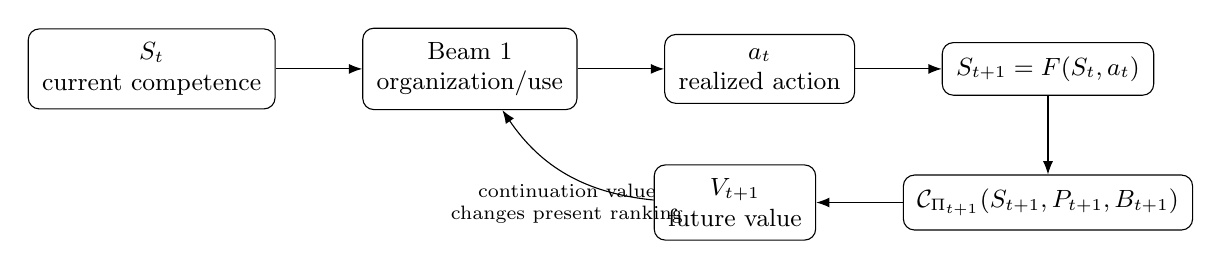
\begin{tikzpicture}[>=Latex,node distance=10mm and 11mm,
 box/.style={draw,rounded corners,align=center,inner sep=5pt,font=\small}]
\node[box] (s) {$S_t$\\current competence};
\node[box,right=of s] (org) {Beam 1\\organization/use};
\node[box,right=of org] (a) {$a_t$\\realized action};
\node[box,right=of a] (sp) {$S_{t+1}=F(S_t,a_t)$};
\node[box,below=of sp] (cap) {$\Ccap_{\Pi_{t+1}}(S_{t+1},P_{t+1},B_{t+1})$};
\node[box,left=of cap] (val) {$V_{t+1}$\\future value};
\draw[->] (s)--(org);
\draw[->] (org)--(a);
\draw[->] (a)--(sp);
\draw[->] (sp)--(cap);
\draw[->] (cap)--(val);
\draw[->,bend left=25] (val) to node[below,align=center,font=\scriptsize]{continuation value\\changes present ranking} (org);
\end{tikzpicture}
\caption{Minimal HLS organization--development cycle. The return arrow is decisional, not backward physical causation.}
\label{fig:hls}
\end{figure}

The architecture distinguishes three regimes. In \emph{juxtaposition}, Beam 1 and Beam 2 coexist but the future-value term is independent of the present organizational choice. In \emph{sequential composition}, present organization affects future competence and value, but the continuation term does not change an optimal present action. In \emph{decision-relevant coupling}, Eq.~\eqref{eq:decisioncoupling} holds. Coupling is therefore distinct from architectural irreducibility.

The minimal endogenous state is $S_t$. Problem structure $P_t$, constraints $B_t$, and admissible organization $\Pi_t$ may remain exogenous time-indexed conditions unless their evolution itself depends on the history. They enter the state only when required to represent the problem being studied.

\section{Minimal Ground Truths}

The theory is accompanied by deliberately small constructive ground truths. Their purpose is not empirical generalization but logical validation: each isolates a distinction that would otherwise be easy to collapse.

\subsection{G1: static ground truth}

G1 uses two agents and two task types with fixed competence. A restricted policy class, ONE, assigns both task types to one agent; ROUTE may assign them separately. The experiments include homogeneous and dominance nulls, crossed specialization, bicriterion effectiveness--resource cases, geometric-expansion nulls, and a bounded organizational-gain window.

The central result is not that routing is superior. It is that the same competence structure can have zero or positive organizational value depending on problem composition and resource constraints. In the equal-resource crossed-specialization control,
\begin{equation}
\Delta_Y(p)=0.8\min(p,1-p),
\end{equation}
with maximum $0.4$ at $p=0.5$. In a bicriterion control with fixed competence and demand, changing only the budget produces
\begin{equation}
\Delta_Y=0\;\rightarrow\;\Delta_Y>0\;\rightarrow\;\Delta_Y=0.
\end{equation}
Thus heterogeneity and attainable-set expansion cannot be identified with realized organizational value.

\subsection{G2: dynamic ground truth}

G2 retains the minimal two-agent/two-task setting and adds endogenous competence change. Three controls establish the dynamic logical chain.

D0 is a null: alternative actions produce identical future states, attainable sets, frontiers, and future values, hence $\Delta^{\mathrm{dev}}=0$.

D1 produces different future competence states and attainable sets, but both efficient frontiers collapse to the same point $(0.8,0.8)$, so $\Delta^{\mathrm{dev}}(p)=0$. Competence change therefore does not imply useful collective-capability change.

D2 produces a genuine present--future trade-off:
\begin{equation}
\Delta R=-0.1,
\qquad
\Delta^{\mathrm{dev}}(p)=0.2p,
\end{equation}
therefore
\begin{equation}
\Delta J(p)=-0.1+0.2p.
\end{equation}
The development-value threshold is $p_V^*=0$, while the decision threshold is
\begin{equation}
p_J^*=0.5.
\end{equation}
Hence positive future development value need not alter the present choice; it becomes decision-relevant only when it exceeds the current operational disadvantage.

Together, G1 and G2 support the complete sequence
\begin{equation}
\begin{split}
\text{heterogeneity}
&\not\Rightarrow \text{organizational value},\\
\text{competence change}
&\not\Rightarrow \text{collective-capability change},\\
\text{capability change}
&\not\Rightarrow \text{useful future value},\\
\text{future value}
&\not\Rightarrow \text{present-decision change}.
\end{split}
\label{eq:nullchain}
\end{equation}
The positive controls show that every transition can also be consequential under the appropriate conditions.

\section{What HLS Adds}

The scientific object of HLS is not any individual component in isolation. Static assignment can be solved with established operations-research tools; competence evolution can be modeled using established learning, training, transfer, or human-capital mechanisms; and dynamic choices can be solved by dynamic programming or stochastic control when those tools apply.

HLS contributes the architecture in which these pieces answer one collective question. It enforces a common capability semantics before and after competence evolution, makes realized organizational action the causal interface to competence change, and separates physical change, collective-capability change, future value, and present decision relevance. This allows a modeler to determine which dependencies are essential in a given HLS instance and which can be removed without changing the scientific question.

This perspective also gives null results a constructive role. A richer organization that does not improve relevant collective capability is evidence of organizational sufficiency, not a failed HLS instance. Competence evolution that does not change future value is a dynamic null, not evidence that learning did not occur. A positive development value that does not change the present action identifies sequential interaction without decision-relevant coupling. The framework therefore supports principled reduction as well as richer models.

The resulting research program is broader than the foundational model. Beam 2 can later instantiate explicit teachers, transfer networks, deliberate training, forgetting, uncertainty, or resource competition. Beam 1 can instantiate richer routing, collaboration, hierarchy, or distributed coordination. These mechanisms should be introduced only when the scientific question requires them. The foundation itself remains the two-operator architecture of Fig.~\ref{fig:hls}.

\section{Discussion}

Three boundaries are especially important.

First, HLS does not claim that heterogeneity is intrinsically valuable. Its value depends on whether organization can expose relevant comparative capability under actual problems and constraints.

Second, HLS does not claim that competence development is intrinsically valuable. Development matters only through future collective capability and the problems for which that capability is useful.

Third, decision-relevant coupling does not imply irreducible centralized management. Future work may characterize what continuation information, prices, contracts, sufficient statistics, or coordination mechanisms allow modular components to reproduce an integrated optimum. That is an architectural question beyond the minimal T0--T6 foundation.

These boundaries also clarify the role of applications. Human organizations, multi-model AI systems, mixtures of specialized learners, autonomous-agent collectives, and skill-based service systems may instantiate very different $S$, $P$, $B$, $\Pi$, and $F$. HLS does not require them to share a learning mechanism. It requires only that their distributed competences, organizational accessibility, and endogenous competence evolution can be represented without collapsing the distinctions in Eq.~\eqref{eq:nullchain}.

\section{Conclusion}

Heterogeneous Learning Systems studies a collective with distributed and evolving competences through two linked questions: who should do what, and who should learn what, how, and from whom. The minimal theory requires neither a new assignment formalism nor a new theory of learning or dynamic optimization. It requires a common collective-capability operator, an endogenous competence transition driven by realized action, and the reuse of the former on the future competence state.

This structure makes explicit a sequence of distinctions that are easily conflated: heterogeneity, attainable capability, efficient capability, realized organizational value, competence change, future collective value, and decision relevance. Minimal static and dynamic ground truths validate both the null and positive cases. The resulting HLS foundation is therefore intentionally compositional: established theories are imported wherever they suffice, while the HLS architecture determines how they fit together and what must be measured or proved for their interaction to become consequential.

\printbibliography
\end{document}
